
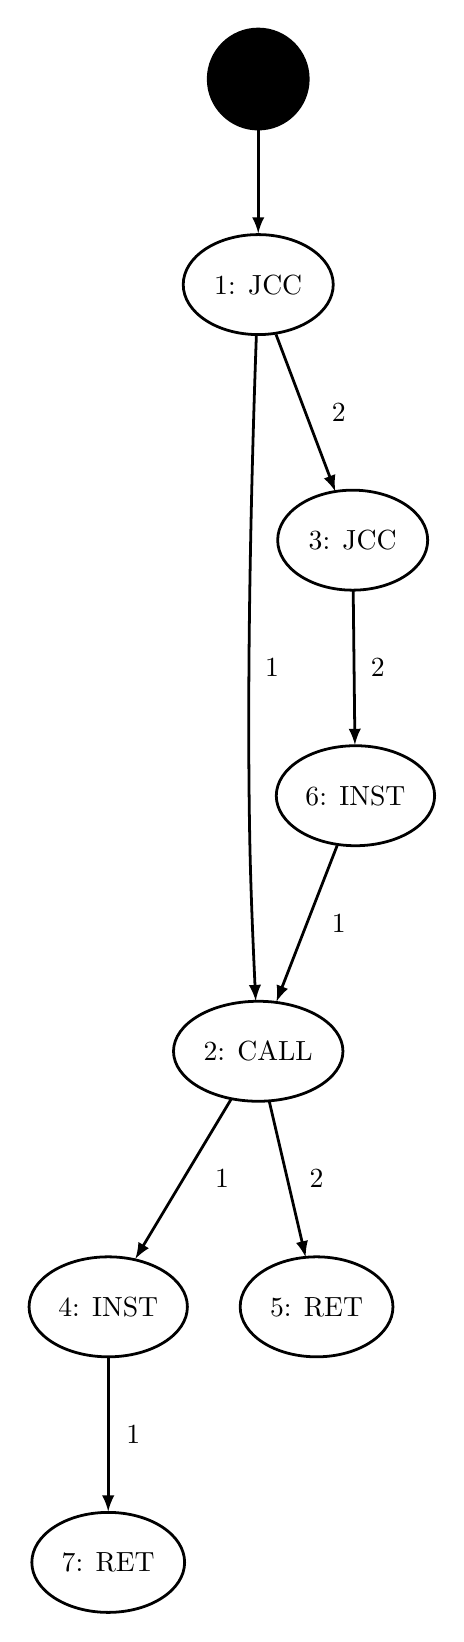
\begin{tikzpicture}[>=latex,line join=bevel,]
  \pgfsetlinewidth{1bp}
%%
\pgfsetcolor{black}
  % Edge: 2 -> 3
  \draw [->] (73.346bp,184.91bp) .. controls (65.18bp,171.3bp) and (53.344bp,151.57bp)  .. (38.753bp,127.25bp);
  \definecolor{strokecol}{rgb}{0.0,0.0,0.0};
  \pgfsetstrokecolor{strokecol}
  \draw (70.0bp,156.0bp) node {1};
  % Edge: 6 -> 7
  \draw [->] (117.19bp,367.65bp) .. controls (117.34bp,354.82bp) and (117.53bp,337.11bp)  .. (117.81bp,312.3bp);
  \draw (126.0bp,340.0bp) node {2};
  % Edge: 1 -> 6
  \draw [->] (89.395bp,460.07bp) .. controls (94.413bp,446.79bp) and (101.48bp,428.07bp)  .. (110.75bp,403.55bp);
  \draw (112.0bp,432.0bp) node {2};
  % Edge: 7 -> 2
  \draw [->] (111.42bp,276.07bp) .. controls (106.28bp,262.87bp) and (99.064bp,244.31bp)  .. (89.554bp,219.85bp);
  \draw (112.0bp,248.0bp) node {1};
  % Edge: 1 -> 2
  \draw [->] (82.332bp,459.79bp) .. controls (81.075bp,425.05bp) and (78.603bp,344.04bp)  .. (80.0bp,276.0bp) .. controls (80.31bp,260.89bp) and (80.982bp,244.03bp)  .. (82.098bp,220.1bp);
  \draw (88.0bp,340.0bp) node {1};
  % Edge: 0 -> 1
  \draw [->] (83.0bp,533.94bp) .. controls (83.0bp,525.81bp) and (83.0bp,515.88bp)  .. (83.0bp,496.44bp);
  % Edge: 2 -> 5
  \draw [->] (86.95bp,184.07bp) .. controls (90.0bp,171.0bp) and (94.279bp,152.66bp)  .. (100.07bp,127.85bp);
  \draw (104.0bp,156.0bp) node {2};
  % Edge: 3 -> 4
  \draw [->] (29.0bp,91.647bp) .. controls (29.0bp,78.823bp) and (29.0bp,61.108bp)  .. (29.0bp,36.3bp);
  \draw (38.0bp,64.0bp) node {1};
  % Node: 1
\begin{scope}
  \definecolor{strokecol}{rgb}{0.0,0.0,0.0};
  \pgfsetstrokecolor{strokecol}
  \draw (83.0bp,478.0bp) ellipse (27.0bp and 18.0bp);
  \draw (83.0bp,478.0bp) node {1: JCC};
\end{scope}
  % Node: 0
\begin{scope}
  \definecolor{strokecol}{rgb}{0.0,0.0,0.0};
  \pgfsetstrokecolor{strokecol}
  \definecolor{fillcol}{rgb}{0.0,0.0,0.0};
  \pgfsetfillcolor{fillcol}
  \filldraw [opacity=1] (83.0bp,552.0bp) ellipse (18.0bp and 18.0bp);
\end{scope}
  % Node: 3
\begin{scope}
  \definecolor{strokecol}{rgb}{0.0,0.0,0.0};
  \pgfsetstrokecolor{strokecol}
  \draw (29.0bp,110.0bp) ellipse (28.5bp and 18.0bp);
  \draw (29.0bp,110.0bp) node {4: INST};
\end{scope}
  % Node: 2
\begin{scope}
  \definecolor{strokecol}{rgb}{0.0,0.0,0.0};
  \pgfsetstrokecolor{strokecol}
  \draw (83.0bp,202.0bp) ellipse (30.5bp and 18.0bp);
  \draw (83.0bp,202.0bp) node {2: CALL};
\end{scope}
  % Node: 5
\begin{scope}
  \definecolor{strokecol}{rgb}{0.0,0.0,0.0};
  \pgfsetstrokecolor{strokecol}
  \draw (104.0bp,110.0bp) ellipse (27.5bp and 18.0bp);
  \draw (104.0bp,110.0bp) node {5: RET};
\end{scope}
  % Node: 4
\begin{scope}
  \definecolor{strokecol}{rgb}{0.0,0.0,0.0};
  \pgfsetstrokecolor{strokecol}
  \draw (29.0bp,18.0bp) ellipse (27.5bp and 18.0bp);
  \draw (29.0bp,18.0bp) node {7: RET};
\end{scope}
  % Node: 7
\begin{scope}
  \definecolor{strokecol}{rgb}{0.0,0.0,0.0};
  \pgfsetstrokecolor{strokecol}
  \draw (118.0bp,294.0bp) ellipse (28.5bp and 18.0bp);
  \draw (118.0bp,294.0bp) node {6: INST};
\end{scope}
  % Node: 6
\begin{scope}
  \definecolor{strokecol}{rgb}{0.0,0.0,0.0};
  \pgfsetstrokecolor{strokecol}
  \draw (117.0bp,386.0bp) ellipse (27.0bp and 18.0bp);
  \draw (117.0bp,386.0bp) node {3: JCC};
\end{scope}
%
\end{tikzpicture}

